\chapter{XXX对XXXX的影响}\label{chap:ch2}

本段为章前导语，主要用于对本章研究内容进行简要引入与概括说明。通常可包括本章研究目的、主要研究内容、拟解决的问题以及章节结构安排等，以增强章节之间的衔接性和整体逻辑性。

\section{材料与方法}\label{sec:ch2-methods}

\subsection{材料与试剂}\label{subsec:ch2-materials}

本节用于填写试验原料来源、主要化学试剂名称、纯度等级、生产厂家及批次信息等。

\subsection{仪器与设备}\label{subsec:ch2-instruments}

本节用于填写主要实验仪器、型号、生产厂家及关键测试设备信息。

\subsection{XXXX的制备}\label{subsec:ch2-preparation}

本节用于描述样品制备、处理条件设置及工艺流程。

\subsection{XXXX的测定}\label{subsec:ch2-determination}

本节用于描述指标测定方法、计算公式和操作要点。

例如，综合指标的计算过程可写为：
\begin{align}
	Z_i &= \sum_{j=1}^{n}\omega_j z_{ij} \\
	z_{ij} &= \frac{x_{ij}-\bar{x}_j}{s_j} \\
	s_j &= \sqrt{\frac{1}{m-1}\sum_{i=1}^{m}\left(x_{ij}-\bar{x}_j\right)^2}
	\label{eq:ch2-example}
\end{align}

式中，$Z_i$ 表示第 $i$ 个样品的综合得分；$\omega_j$ 表示第 $j$ 个指标的权重；$z_{ij}$ 表示标准化后的指标值；$\bar{x}_j$ 表示第 $j$ 个指标的平均值；$s_j$ 表示标准差。

\subsection{统计与分析}\label{subsec:ch2-statistics}

本节用于说明试验重复次数、统计方法与绘图软件等。

\section{结果与讨论}\label{sec:ch2-results}

\subsection{XXXXXXXXX}\label{subsec:ch2-result-a}

本部分用于展示研究结果，并结合相关理论与文献对结果进行分析讨论，阐明其变化规律、影响因素及可能作用机制。涉及上下标、公式、变量符号及统计学表达时，建议采用规范的 \LaTeX{} 数学格式书写，如$\mathrm{O}_2^{\cdot-}$、$k_{\mathrm{cat}}$、$R^2$、$p<0.05$、$\Delta E$、$\mu\mathrm{m}$、$10^{-3}$、$a_i^{(n)}$、$\mathrm{PPO}_{\mathrm{activity}}$等。

\begin{center}
	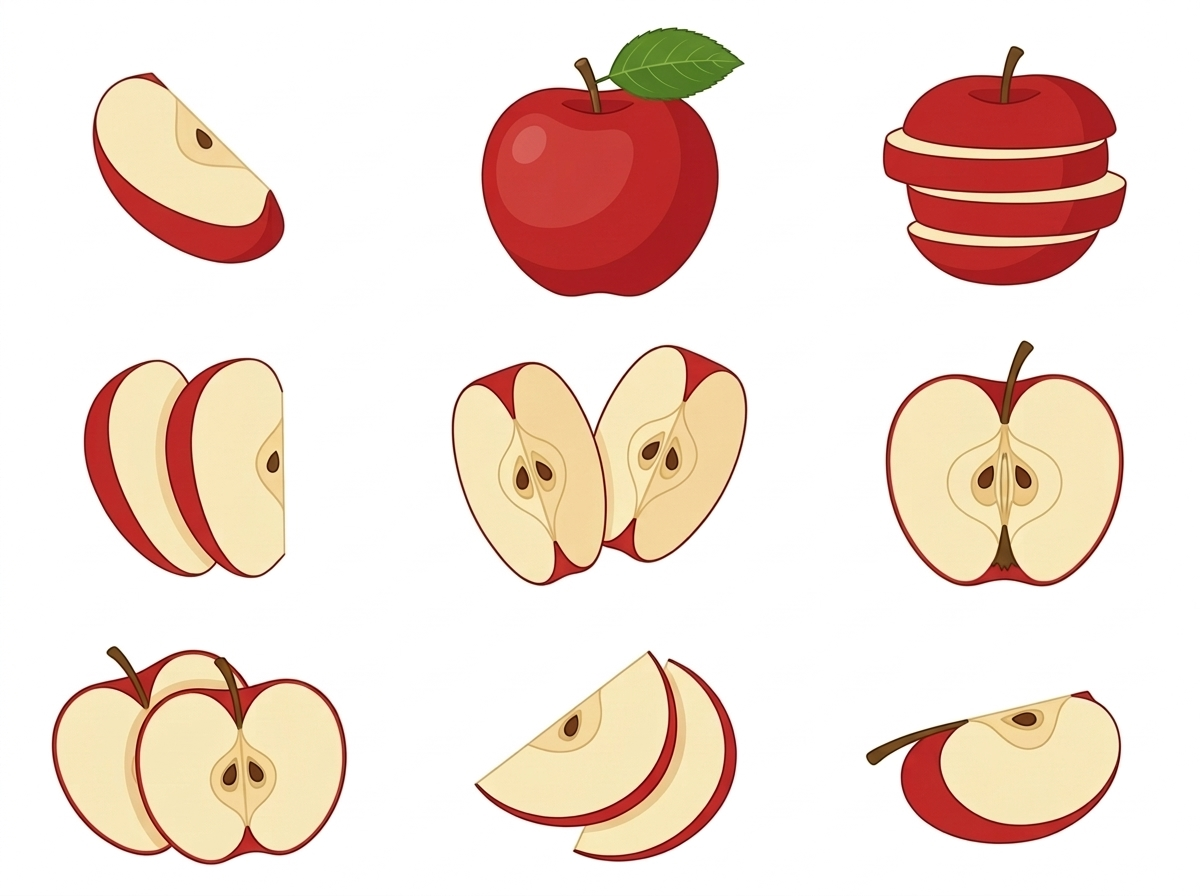
\includegraphics[width=0.6\textwidth]{figures/apple.png}
	\captionof{figure}[XXXX变化趋势]{XXXX变化趋势。\par
		（A）XXXX；（B）XXXX；（C）XXXX。\par
		注：不同小写字母代表存在显著差异（$p<0.05$）。\par
		{\qauTimes\fontsize{10.5bp}{15.75bp}\selectfont \textbf{Fig.~\thefigure\ Trend of XXXX changes.}}\par
		{\qauTimes\fontsize{10.5bp}{15.75bp}\selectfont \textbf{(A) XXXX; (B) XXXX; (C) XXXX.}}\par
        {\qauTimes\fontsize{10.5bp}{15.75bp}\selectfont \textbf{Different lowercase letters indicate significant differences (\boldmath$p<0.05$).}}}
	\label{fig:ch2-example}
\end{center}

\subsection{XXXXXXXXX}\label{subsec:ch2-result-b}

本部分用于展示研究结果，并结合相关理论与文献对结果进行分析讨论，阐明其变化规律、影响因素及可能作用机制。涉及上下标、公式、变量符号及统计学表达时，建议采用规范的 \LaTeX{} 数学格式书写，如$\mathrm{O}_2^{\cdot-}$、$k_{\mathrm{cat}}$、$R^2$、$p<0.05$、$\Delta E$、$\mu\mathrm{m}$、$10^{-3}$、$a_i^{(n)}$、$\mathrm{PPO}_{\mathrm{activity}}$等。

\begin{center}
	\captionof{table}[示例表题：不同处理下指标测定结果]{不同处理下指标测定结果\par
		{\qauTimes\fontsize{10.5bp}{15.75bp}\selectfont \textbf{Table~\thetable\ Determination results of different indices under different treatments}}}
	\label{tab:ch2-example}
	\renewcommand{\arraystretch}{1.5}
	{\songti\zihao{5}
		\begin{tabular*}{0.85\textwidth}{@{\extracolsep{\fill}}>{\centering\arraybackslash}m{0.18\textwidth}>{\centering\arraybackslash}m{0.26\textwidth}>{\centering\arraybackslash}m{0.26\textwidth}}
			\toprule
			处理 & 指标 1 & 指标 2 \\
			\midrule
			CK & 0.00$\pm$0.00\textsuperscript{a} & 0.00$\pm$0.00\textsuperscript{a} \\
			T1 & 0.00$\pm$0.00\textsuperscript{b} & 0.00$\pm$0.00\textsuperscript{ab} \\
			T2 & 0.00$\pm$0.00\textsuperscript{c} & 0.00$\pm$0.00\textsuperscript{b} \\
			\bottomrule
		\end{tabular*}
		\par
		{\center 注：不同小写字母代表存在显著差异（$p<0.05$）。\par}
	}
\end{center}

\section{小结}\label{sec:ch2-summary}

本节用于归纳本章主要结果，概括关键发现并为下一章研究奠定基础。
